\documentclass[../thesis.tex]{subfiles}
\begin{document}

\begin{figure*} [t]
 \centering
            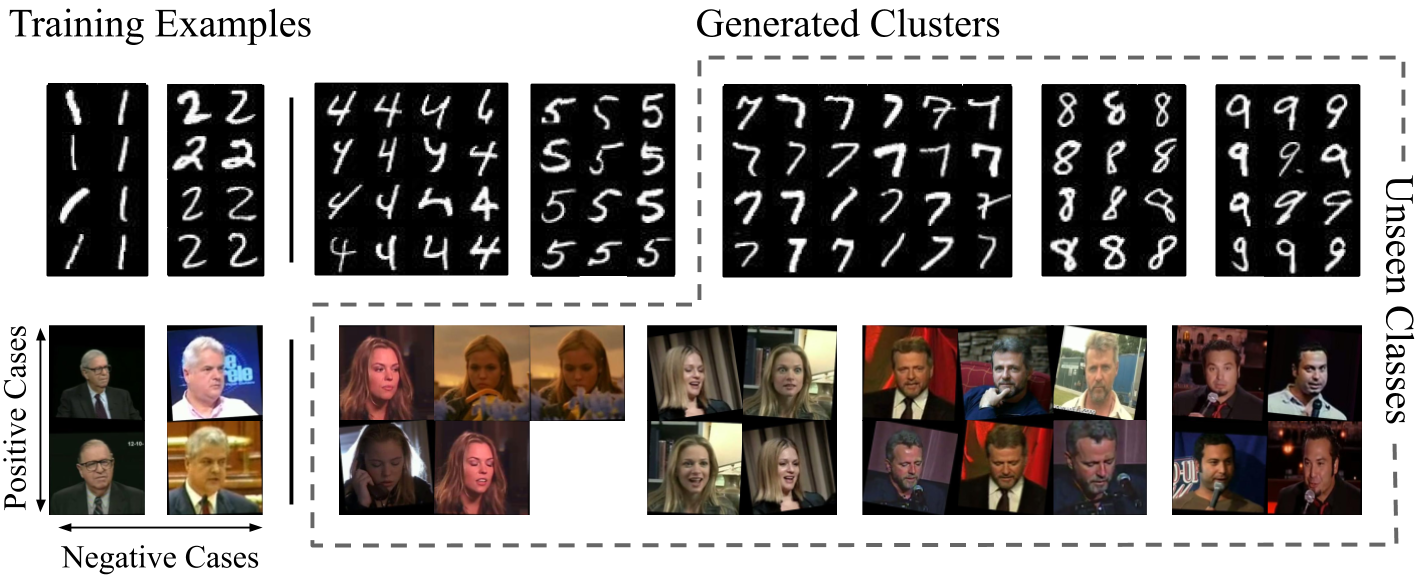
\includegraphics[width=0.9\linewidth]{../files/DMS/images/unseen_discovery_2_rows.png}
             \caption{Examples of learnt clusters given side-information.
             Positive examples contain two data points known to be from the same class and negative examples are from different classes. Here, the same class is either the same digit (top) or the same person (bottom) and negative examples are of two different classes. Our method learns to correctly identify unseen classes. For example, the 7, 8, and 9 clusters are not present when training on MNIST (top).}
             \vspace{-5mm}
    \label{fig__DMS__teaser}
 \end{figure*}  
 
\section{Introduction}
The ability to identify repetition is one of the two key components of counting, alongside object detection.
In this chapter, we address this repetition recognition independently of detection by framing it as a clustering task.
Clustering, also known as cluster analysis, involves the process of organising a collection of items in a manner that items within the same cluster exhibit greater resemblance to one another than they do to items in different clusters.
Automated clustering is one of the fundamental problems in machine learning due to its varied use cases and minimal requirement for labelling.
Unlike classification, most clustering methods group data points by type with little to no supervision and no ground-truth class labels.
This enables them to operate in a class-agnostic way. They can discover previously unseen classes and be utilised in applications where there is limited labelled data available. 

As discussed in \Cref{sec__litreview__clustering}, to separate data points correctly, classical clustering approaches normally require some kind of general holistic information about the data. This can take various forms, but most commonly it revolves around either a known number of clusters as in algorithms like $k$-means \cite{Lloyd1982} and DBSCAN \cite{Sander1998} or a predefined boundary for a proxy similarity metric, as in methods like mean shift \cite{Fukunaga1975}. 
Usually, this proxy is a simple metric, such as the L$_1$, Euclidean, or Cosine distance, in an embedded feature space.
In many real-world cases, the exact number of clusters may be unknown, and it is often difficult to specify an informative distance tolerance to separate intra-class variation from inter-class variation. 
Defining an informative proxy similarity metric is especially difficult in high-dimensional or complex feature spaces since the usual metrics scale poorly with dimensionality.
These simple metrics inherently prioritise the feature dimensions with the greatest magnitude variation, meaning they will always group the same data in the same, `most obvious', way.

While datasets generally provide a single label per image, it is clear that many datasets could be clustered in multiple valid ways.
We refer to the `most obvious' clustering task of a dataset, which is usually the task the labels refer to, as the \textit{intrinsic} task, and the other valid divisions as the \textit{non-intrinsic} task; examples of possible non-intrinsic tasks are presented in \Cref{fig__intrisic_non_intrinsic}. This is closely linked to the idea we proposed in \Cref{sec__lit_rev__count_valid_but_unkonwon_counts} of valid-but-unknown counts.
Up to this point, clustering methods generally focus on identifying intrinsic tasks and have little to no ability to perform non-intrinsic clustering, \ie finding groupings where the most salient features do not have the greatest variance.

At the time of writing this work, deep-learning-based methods used these classical algorithms either to supervise their training \cite{Shah2018,shah2018deep} or to directly cluster a projected feature space which has been optimised for the task at hand \cite{Chang2017, Yang2017}. These approaches suffer from the same problems as their respective classical methods and generally require significant parameter tuning.

In this chapter, we propose Differentiable Mean Shift (DMS), a method inspired by both work that uses pairwise similarity-based side-information to cluster data \cite{xing2002distance,han2020automatically, Han} and mean-shift \cite{Fukunaga1975}, an iterative clustering algorithm which uses a Euclidean distance metric as a proxy for similarity.
DMS is the natural progression of these two approaches.
It removes the overly simplistic similarity proxy of Euclidean distance of the original mean-shift algorithm and instead uses side-information to learn a task-specific similarity kernel.
This kernel identifies the features salient to a specific task, generating an understanding of the clusters directly from the side-information. 
We believe that using side-information in the form of choosing a small set of `similar' or `dissimilar' pairs is more intuitive and easier for a user than defining an abstract distance tolerance in an embedded feature space and also works in use cases where the number of clusters is not known by an end-user.

We train the differentiable kernel to evaluate the similarity of a given pair of points in the context of a specific task.
It adjusts its understanding of the importance of different aspects of the data, learning a task-specific definition of what it means to be within the same cluster. 
Because of this, DMS can accurately cluster the same dataset in multiple valid ways depending on the side-information provided.

DMS is able to generate accurate clusters without the need for either a clustering-specific embedded feature space; dataset-specific hyper-parameter tuning present in other methods \cite{Hsu2015, Liu2015, Ceccarelli2008, Li2018}; a  wider knowledge of the dataset such as the number of clusters, their centres, or their spatial distribution; or even all of the classes to be present during training.
As our method operates as a single forward pass through a lightweight network which does not require hyper-parameter tuning, dimensionality reduction, or an understanding of the whole dataset, it is trivial to include it within another deep learning method either as a final head or integrated into the end-to-end training of another task. We do not train backbones or feature encoders; instead, we operate on the input data features directly.

In this chapter, we show that our method outperforms prior
approaches in both the intrinsic and non-intrinsic dataset tasks, that it is possible to train a strong cluster definition without enforcing a constraint that each cluster must be presented during training, and that the learnt definition is flexible, learning various clustering tasks from side-information alone.
This accuracy and flexibility paired with the lightweight nature of the network make DMS well-suited to various deployment situations.

Our main contributions are:
\begin{itemize}
    \item A new approach to clustering, which directly clusters points trained using only side-information rather than using distance tolerances, a known number of clusters, or any other laborious hyper-parameter tuning.
    \item A differentiable, mean-shift-inspired framework that can be easily added to other machine learning methods.
    \item A state-of-the-art algorithm that outperforms other contemporary methods on intrinsic tasks and is capable of performing non-intrinsic task clustering on various datasets.
\end{itemize}

The remainder of this chapter is structured as follows. 
\Cref{sec__DMS__DMS} outlines and formalises the mathematics of the classical mean shift algorithm and our differentiable mean shift process.
\Cref{sec__DMS__experiments} discusses the details of our method and evaluates it in the context of other recent clustering approaches.
We then validate sections of our method in \Cref{sec__DMS__ablation}.


\section{Method}\label{sec__DMS__DMS}
In this section, we outline the formulation of the task of clustering and summarise the original mean shift algorithm. We then outline our proposed method, DMS, which is a fully differentiable, neural network-based method.
Finally, we explain our use of side-information during training and how this facilitates task-specific clustering.

\subsection{Clustering Problem Definition}
Clustering algorithms aim to group a set of $n$, $d$ dimensional points $\{\mathbf{x}_1, \mathbf{x}_2, ..., \mathbf{x}_n\} = \mathcal{X}$ into $k \leq n$ sets $\{S_1, S_2, ... S_k\} = \mathcal{S}$, with centres $\{\boldsymbol{\mu}_1, \boldsymbol{\mu}_2, ..., \boldsymbol{\mu}_k\} = \mathcal{M}$. 

\begin{equation}
    \boldsymbol{\mu}_i = {\frac {1}{|S_{i}|}}\sum _{\mathbf {x} \in S_{i}}\mathbf {x}
\end{equation} 
where $|S_{i}|$ is the number of points in the $i^{th}$ cluster, $S_{i}$. 


\subsection{Mean Shift Kernel}\label{sec__DMS__MS_diff_kernel}
The mean shift algorithm, as presented in \Cref{alg__DMS__meanshift} in \Cref{sec__litreview__meanshift}, iteratively improves an estimate, $\bar {\boldsymbol{\mu}}_i$, of each cluster centre.
This is achieved by finding inlier predictions using the current estimate of the cluster centre and a similarity kernel, $K(.)$.
\begin{equation}\label{eq__DMS__mean_shift_second_time}
    \bar {\boldsymbol{\mu}}^{(n+1)}_i = m(\mathcal{X}, \bar {\boldsymbol{\mu}}^{(n)}_i) = \frac{\sum_{\mathbf x \in \mathcal X} \mathbf x K(\mathbf x, \bar {\boldsymbol{\mu}}^{(n)}_i) }{\sum_{\mathbf x \in \mathcal X} K(\mathbf x, \bar{\boldsymbol{\mu}}^{(n)}_i)},
\end{equation}
\myequations{Mean-Shift Iteration}

In the original mean shift formulation, the Euclidean distance flat kernel $K_F(.)$ was used.
This is defined as a $\lambda\text{-ball} \in \mathbb R^d$ centred at the current estimated cluster mean $\bar{\boldsymbol{\mu}}$, where $d$ is the dimensionality of the feature space. Points within this ball are considered inliers to the cluster.
 
\begin{equation}
    K_F(\mathbf x_1, \mathbf x_2)=
    \begin{cases}
      1 & \text{if}\ \|\mathbf x_1 - \mathbf x_2\|_2 \leqslant \lambda \\
      0 & \text{if}\ \|\mathbf x_1 - \mathbf x_2\|_2 \geqslant \lambda
    \end{cases}
\end{equation}
\myequations{Flat Mean Shift Kernel}
$K_F(.)$ has a strong neighbourhood constraint making it easy to implement and fast to run, but it is not differentiable and requires a good knowledge of the spread of points within each cluster.
Other commonly used similarity kernels are the unit Gaussian Kernel, $K_G$,  and the truncated unit Gaussian kernel, $K_{T}$,  \cite{Cheng1995}. 
\begin{equation}
    K_G(\mathbf x_1, \mathbf x_2)=\frac{1}{\sqrt{2\pi} \sigma^d}\mathbf{e}^{-\frac{\|\mathbf x_1 - \mathbf x_2\|^2}{2\sigma^2}}
\end{equation}
\myequations{Gaussian Mean Shift Kernel}
\begin{equation}
    K_{T}(\mathbf x_1, \mathbf x_2)=
    \begin{cases}
      \beta K_G(\mathbf x_1, \mathbf x_2) & \text{if}\ \|\mathbf x_1 - \mathbf x_2\|_2 \leqslant \lambda \\
      0 & \text{if}\ \|\mathbf x_1 - \mathbf x_2\|_2 \geqslant \lambda
    \end{cases}
\end{equation}
\myequations{Truncated Gaussian Mean Shift Kernel}
Since the Gaussian Kernel has no discrete neighbourhood characteristic, all points in $\mathcal X$ affect the next centre prediction.
However, $K_G$ scales the impact of various points based on their estimated inlier-ship to the current cluster, where inlier-ship is based solely on Euclidean distance. 
While the Gaussian Kernel is differentiable, its representation capabilities are limited as it is symmetrical in all dimensions. 
While this could be improved by having a learnt scaling of different dimensions based on some other metric, it would still scale poorly to more complex feature spaces as the Euclidean distance does not generalise well to higher dimensions.

\subsection{DMS Kernel}
Instead of using Euclidean distance as a proxy for similarity, we propose a differentiable kernel based on a neural network, $K_D$,
which learns to predict similarity more directly. 
The differentiable kernel $K_D(.)$ produces a probability score, predicting the level of similarity between either two arbitrary data points, $(\mathbf{x}_1, \mathbf{x}_2)$, or a data point and an estimated sample mean, $(\mathbf{x}, \bar {\boldsymbol{\mu}})$. The more similar the points, the closer the output of $K_D(.)$ is to 1. Due to the flexibility of the neural network architecture, $K_D(.)$ can learn a deeper understanding of the specific task and, as such, can give more informed predictions of similarity than the classical analytical metrics, such as the aforementioned flat or Gaussian kernels. 
A single $K_D$ similarity prediction is presented visually in \Cref{fig__DMS__Architecture}.


\begin{figure}
        \centering
        \begin{subfigure}{\linewidth}
            \centering
            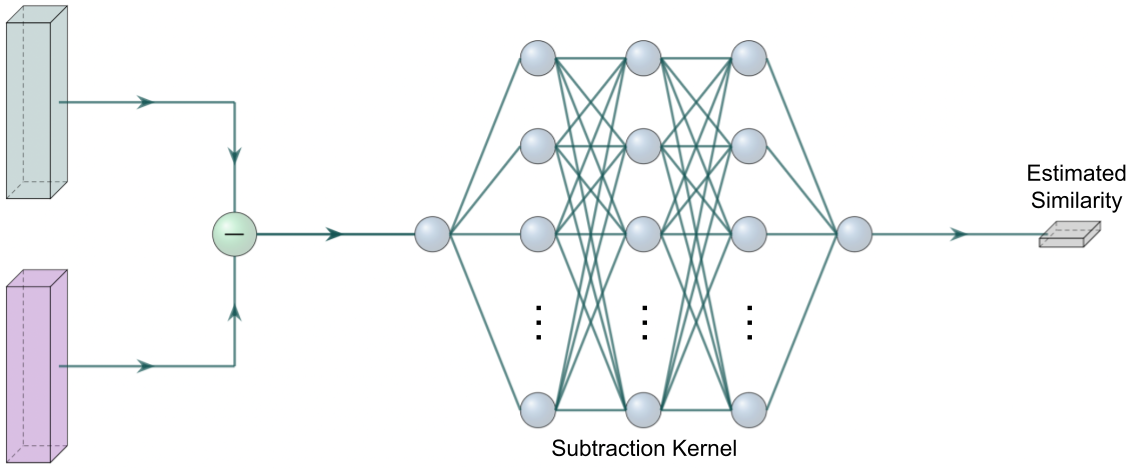
\includegraphics[width=0.81\linewidth]{../files/DMS/images/Dphil_corrections_DMS_Kernel_sub-2.png}
            \caption{Subtraction-Based}
        \end{subfigure}
        \begin{subfigure}{0.82\linewidth}
            \centering
    
            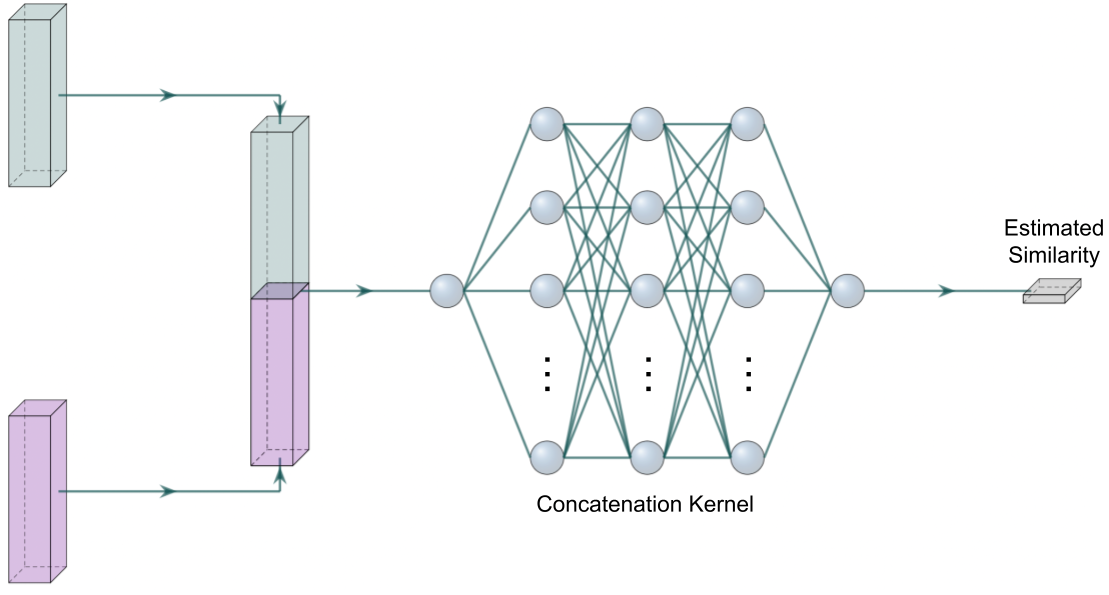
\includegraphics[width=\linewidth]{../files/DMS/images/Dphil_corrections_DMS_Kernel_conv-2.png}
            \caption{Concatenation-Based}
        \end{subfigure}
        \caption{The DMS kernel predicts the similarity of two points from either (a) the difference of their features or (b) their concatenated features.
        All of the latent layers have batch normalisation and ReLu activations. The final layer utilises a sigmoid.}
    \label{fig__DMS__Architecture}
 \end{figure} 


In high-dimensional spaces,  it is often desirable to act non-isotropically across a feature space's dimensions based on a task's requirements. This would help in cases where a dimension has the largest variance but the desired task is invariant to this variation. For example, clustering tasks which focus on semantic class should be invariant to changes in brightness, rotations, or translations. 
A neural network is ideal for these applications as each dimension can be acted on independently to find those most salient to a given task. 
In contrast, since simpler metrics, such as the Euclidean norm, are not able to apply the same contextual knowledge of the feature space, always evaluate dimensions with greater absolute variation as more significant.
This ability of neural networks decreases the need for explicit dimensionality reduction and removes the problems of poor representation inherent in such a reduction.
The context-based dimensional independence also allows a single feature space to be clustered differently depending on the task.



The latent layers of $K_D$ have rectified linear activations applied, and the output of $K_D$ is bounded to $[0,1]$ by a sigmoid function.
\begin{equation}
    \mathrm{Sig}(x)= \frac {1}{1+e^{-x}}
\end{equation}
\myequations{Sigmoid Function}
These activations provide non-linearities to the feature space allowing for much greater complexity of analysis as well as scaling the results to more closely resemble the behaviour of the traditional Gaussian kernel, increasing and decreasing the impacts of the areas close to and far from the sample mean respectively.





\subsection{DMS Algorithm}

    \begin{figure*}[t] 
    \centering
                   \begin{subfigure}{0.32\linewidth}
            \centering
            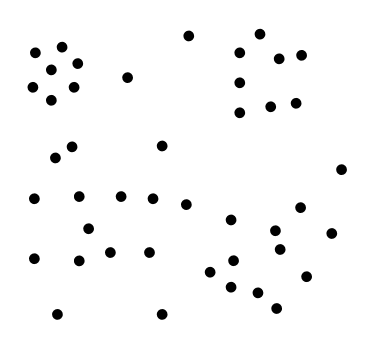
\includegraphics[width=\linewidth]{../files/DMS/images/cluster_how_to_a.png} 
            \caption*{Data Points}
            \end{subfigure}
            \begin{subfigure}{0.32\linewidth}
            \centering
            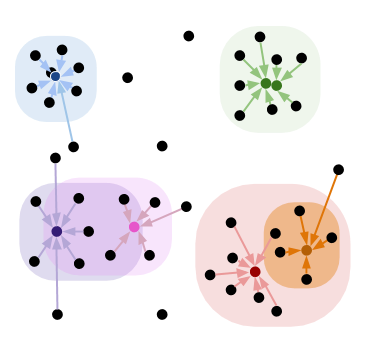
\includegraphics[width=\linewidth]{../files/DMS/images/cluster_how_to_b-4.png} 
            \caption*{Centre Finding Stage }
            \end{subfigure}
                \begin{subfigure}{0.32\linewidth}
            \centering
            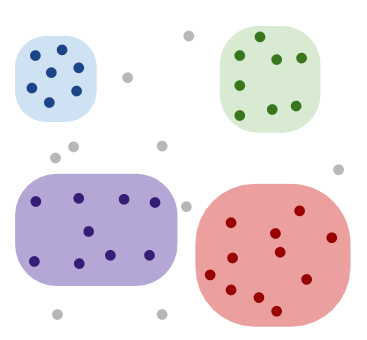
\includegraphics[width=\linewidth]{../files/DMS/images/cluster_how_to_c_2.png} 
            \caption*{Inlier Prediction Stage}
            \end{subfigure}
          \caption{Algorithm Stages. First, the centres are located with an initial approximation of the clusters. Then, given the centres, inliers are found, the clusters are refined, similar clusters are combined, subset clusters are incorporated, and noise points are removed.}
        \label{fig__DMS__process}
    \end{figure*}


\begin{algorithm}
\caption{The DMS Algorithm}\label{alg__DMS__DMS}

\begin{algorithmic}
\Function{DMS}{$\mathcal{X}$}
\State ${\mathcal{X}}_{init} \in \mathcal{X}$, select a set of initialisation points 
\ForEach{point $\mathbf{x}_i \in \mathcal{X}_{init}$}
    \State $\bar{\boldsymbol{\mu}}_i$ = findCentre($\mathbf{x}_i$, $\mathcal{X}$)

\EndFor
\State $\mathcal{M} = \{\mu_0, \mu_1, ..., \mu_i, ...\}$, the set of all estimate centres


\State $\mathcal{M}$ = combineCentres($\mathcal{M}$, $\mathcal{X}$, $\tau$), remove duplicate centres

\ForEach{point $\mathbf{x}_i \in \mathcal{X}$}


    \State $\hat{S}(i) = \underset{j}{\mathrm{argmax}} 
       (K_D(\mathbf{x}_i, \hat{\boldsymbol{\mu}}_j))$, find the most confident cluster

    \If{$K_D(\mathbf{x}_i, \hat{\boldsymbol{\mu}}_j) < (1 - \tau)$}
    
        \State $\hat{S}(i)$ = outlier, if no clusters are confident the point is an `outlier'
    \EndIf
\EndFor

\EndFunction
\item[]

\Function{findCentre}{$\mathbf{x}_i$, $\mathcal{X}$}
\State $\bar{\boldsymbol{\mu}}^{(n)}_i = \mathbf{x}_i$
\State$    \bar {\boldsymbol{\mu}}^{(n+1)}_i = m(\mathcal{X}, \bar {\boldsymbol{\mu}}^{(n)}_i) = \frac{\sum_{\mathbf x \in \mathcal X} \mathbf x K(\mathbf x, \bar {\boldsymbol{\mu}}^{(n)}_i) }{\sum_{\mathbf x \in \mathcal X} K(\mathbf x, \bar{\boldsymbol{\mu}}^{(n)}_i)}$

\If{$\frac{1}{|\mathcal X|}\sum_{\mathbf x \in \mathcal X} ||K_D(\mathbf x, \bar{\boldsymbol{\mu}}^{(n)}_i) - K_D(\mathbf x, \bar{\boldsymbol{\mu}}^{(n-1)}_i)|| < 10^{-6}$}
    \State $\bar{\boldsymbol{\mu}}_i = \bar{\boldsymbol{\mu}}^{(n)}_i$
\Else
    \State $\bar{\boldsymbol{\mu}}_i$ = findCentre($\bar {\boldsymbol{\mu}}^{(n+1)}_i$, $\mathcal{X}$, $\tau$)
\EndIf

\EndFunction



\item[]
\Function{combineCentres}{$\mathcal{X}$, $\mathcal{M}$}

\State $\mathbf{H} = [|\mathcal{X}| \times |\mathcal{M}|]$
\State $\mathbf{S} = [|\mathcal{M}|\times |\mathcal{M}|]$
\ForEach{point $\mathbf{x}_i \in \mathcal{X}$}
    \ForEach{centre $\boldsymbol{\mu}_j \in \mathcal{M}$}
        \State $\mathbf{H}_{i,j}=K_D(\mathbf{x}_i, \bar{\boldsymbol{\mu}}_j)$
    \EndFor
\EndFor

\State $\tilde{\mathbf H}$ = biStochasticNormalisation($\mathbf H$) \cite{Coifman_2013}

\State $\mathbf S=\tilde{\mathbf H} \tilde{\mathbf H}^\top > 0.5$
\State Comp = $\{\{i,j,k\}, \{p,q,r\}, ...\{x,y,z\}\}$ = findConnectedComponents($\mathbf S$) \cite{Pearce2005AnIA}

\State $\mathcal{M}$ = $\{\boldsymbol{\mu}_i, \boldsymbol{\mu}_p, ..., \boldsymbol{\mu}_x\}$ = removeDuplicateCentres($\mathcal{M}$, Comp)
 \EndFunction

\end{algorithmic}
\end{algorithm}


Our method, which in practicality is a single pass through a neural network, is comprised of two stages: i) iterative centre finding and ii) refined inlier prediction. 
A visual layout of these stages is shown in \Cref{fig__DMS__process} and \Cref{alg__DMS__DMS} outlines the DMS algorithm in pseudo-code.
During the first stage, the cluster centres are found by iteratively taking the weighted average of their inliers predictions, $K_D(\mathbf x_i, \bar {\boldsymbol{\mu}})$. In the second stage, similar centres are merged. During this conglomeration, two centres are said to be the same if their inlier predictions of all of the points in $\mathcal X$ are similar. The second stage also refines the inlier predictions as well as defining outlier points.


    
To estimate the sample mean vector of a cluster, we initialise $\bar{\boldsymbol{\mu}}^{(0)} = \mathbf x_i$, where $\mathbf{x}_i \in \mathcal X$.   
We then predict the sample mean iteratively, $\bar{\boldsymbol{\mu}}^{(n+1)} = m(\mathcal X, \bar{\boldsymbol{\mu}}^{(n)})$, where $n$ is the iteration step index; one step can be seen in \Cref{fig__DMS__loop_diagram}.
Unlike classical mean shift, we do not determine convergence by defining a distance tolerance between the centres found in consecutive iterations. Instead, we use the prediction of inliers given the current and previous sample mean. If two consecutive sample means, $\bar{\boldsymbol{\mu}}^{(n-1)}$ and  $\bar{\boldsymbol{\mu}}^{(n)}$, predict the same points to be inliers and outliers, the algorithm has converged, and the cluster centre has been found. 
Formally, the algorithm has converged if
    \begin{equation}\label{eq__DMS_convergence}
        \frac{1}{|\mathcal X|}\sum_{\mathbf x \in \mathcal X} ||K_D(\mathbf x, \bar{\boldsymbol{\mu}}^{(n)}_i) - K_D(\mathbf x, \bar{\boldsymbol{\mu}}^{(n-1)}_i)|| < \tau
    \end{equation}
where $\tau$ is the convergence threshold.
In this way, we can calculate $M$ sample means, $\bar{\boldsymbol{\mu}}_i$, initialised from $\mathbf{x}_i$, where $i=1,..,M$.

\begin{figure}
        \centering
        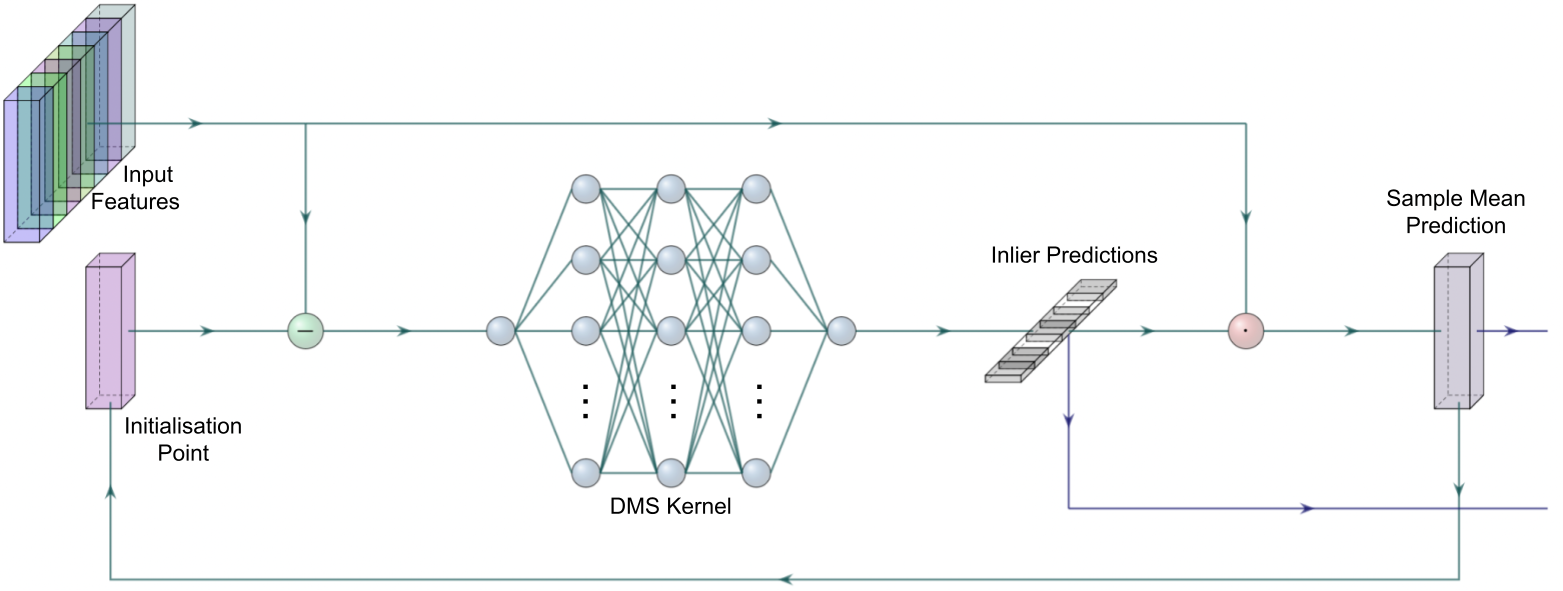
\includegraphics[width=\linewidth]{../files/DMS/images/Dphil_corrections_DMS_pipeline.png}
        
        \caption{The DMS framework for iterative cluster centre finding and inlier prediction.}
    \label{fig__DMS__loop_diagram}
 \end{figure} 

We evaluate sample mean similarity in the same way as iterative convergence. This is necessary because while in most cases similar samples converge to an identical cluster centre, \ie $\|\bar{\boldsymbol{\mu}}_i-\bar{\boldsymbol{\mu}}_j\|_2 < 10^{-6}$, we observe that samples that belong to the same ground-truth cluster frequently converged to different but similar sample means. 
To manage this discrepancy, we define two centres to be the same if both clusters predict the same points to be inliers and outliers with similar confidences.

Formally, we calculate a confidence matrix $\mathbf H\in\mathbb [0,1]^{|\mathcal{X}|\times M}$ where the element $\mathbf H_{i,j}$ represents the confidence that the data point $\mathbf{x}_i$ belongs to the candidate cluster $j$.

\begin{equation}
    \mathbf H_{i,j}=K_D(\mathbf{x}_i, \bar{\boldsymbol{\mu}}_j)
\end{equation}
\myequations{Confidence Matrix}
A prediction similarity matrix over the candidate sample means can be calculated $\mathbf S=\tilde{\mathbf H} \tilde{\mathbf H}^\top$, where $\tilde{\mathbf H}$ is the bi-stochastic normalisation  of $\mathbf H$ \cite{Coifman_2013}. Each element $\mathbf S_{i,j}$ measures the similarity between the sample means $\bar{\boldsymbol{\mu}}_i$ and $\bar{\boldsymbol{\mu}}_j$. 
We find the final unique cluster centres by binarising $\mathbf S$ and extracting the connected components \cite{Pearce2005AnIA}.
The same binarising tolerance $\tau = 0.5$ is used for all datasets. However, we found that any value between $0.1$ and $0.95$ will provide similar results as the values are driven to either $1$ or $0$ by the training loss; see \Cref{eq__DMS__eq_BCE}.
Each data point is then assigned to the cluster with the highest inlier confidence for that point.

\begin{equation}
    \hat{S}(i) =
    \begin{cases}
       \underset{j}{\mathrm{argmax}} 
       (K_D(\mathbf{x}_i, \hat{\boldsymbol{\mu}}_j)) & \text{if\hspace{1em}} K_D(\mathbf{x}_i, \hat{\boldsymbol{\mu}}_j) > (1 - \tau) \\
      \text{outlier} & \text{else}
    \end{cases}
\end{equation}
\myequations{DMS Final Cluster Assignment}
In datasets with high variance, it can be the case that a point which originally converged to a particular centre is not assigned to the associated cluster during the final stage. This is either due to a different centre being more confident of its inliership in the final stage or because no cluster is confident of its inliership. 
Generally, this is desirable, as points not associated with any cluster or on the border of two clusters may converge to an incorrect centre during our first stage due to the lack of a hard neighbourhood constraint in $K_D$.
The most obvious way to understand this is that a trail of data points could gradually lead the predicted mean a greater distance from the initialisation point than another, closer, possible cluster mean that has fewer of these `stepping stone' points.

Following this stage, the clusters could be further refined in various ways. For example, trivial single-point solutions could be removed if it is known that this case does not occur in the data. During our testing, we do not remove these trivial solutions as this implies knowledge of the dataset.

It is worth noting that while classical mean shift needs to be initialised from every point in the dataset, our algorithm only needs to be initialised from at least one point per cluster. Classical mean shift classifies a point as belonging to a cluster if it converges to the associated centre;
our algorithm only needs to find each cluster centre as our second stage finds all inliers of all of the clusters.

\subsection{Training with Side-Information}
During training, we generate data as follows.
A given dataset, $\mathcal X$,  and task configuration contains a set of categories, $\mathcal C$, and each category $c\in\mathcal C$ contains a number of samples, $|c|$. 
This cardinality may vary between categories. 
These category boundaries are task-specific. For example, the categories for dividing by colour will be different from those for dividing by shape.
We divide the dataset into a set of training points, $\mathcal{X}_{tr}$, and evaluation points, $\mathcal{X}_{ev}$, where $\mathcal{X} = \mathcal{X}_{tr} \cup \mathcal{X}_{ev}$. 
We assume that we have side-information in the form of relational 'similar/dissimilar' labels for the points in $\mathcal{X}_{tr}$ but not for those in $\mathcal{X}_{ev}$. 

One training instance is composed of a random data point, $\mathbf{x}$, called the initialisation point, a set of positive samples, $\mathcal P$, a set of negative samples, $\mathcal N$, and a set of unlabelled samples,  $\mathcal U$. 
As the datasets we use include ground-truth labels instead of pairwise side-information, we generate the side-information from the ground-truth labels, then discard the ground-truth labels.
$\mathcal{P}$ is composed of points drawn from the same class as the initialisation point, $\mathcal{N}$ is drawn from the points of different classes to the initialisation point, and $\mathcal U$ is drawn from all points in $\mathcal{X}$.

The specific class labels of all of the points are discarded once these categories, which define the side-information, are created.
The use of pairwise relational labels as side-information instead of using the specific class label during training allows the clustering network to learn a representation of similarity independent of the specific class.

Only points in $\mathcal{X}_{ev}$ are used during testing.
While the unlabelled samples, $\mathcal U$, are taken from the entire dataset, $\mathcal{X}$, they are excluded from the training loss.
The unlabelled data points serve only to increase the cardinality and variance of the clusters during training, facilitating more consistent cluster convergence.
All classes and data points in $\mathcal P$, $\mathcal N$, and $\mathcal U$ are randomly and independently selected. Points can be repeated in a training instance, 
facilitating training in situations where there are not enough available data points
to create sufficiently large positive class sizes.

During training, we use four mean shift iterations; the impact of this is further discussed in \Cref{sec__DMS__ablation}.
We used the Binary Cross Entropy \cite{cox1958regression} 
of the inlier predictions and the side-information of the labelled points as the training loss, see \Cref{eq__DMS__eq_BCE}. Predictions of the unlabelled points are not used in the loss. 
\begin{equation}\label{eq__DMS__eq_BCE}
\text{Loss} = -\sum_{i \in{\mathcal P,\, \mathcal N}} (y_i\log(p_i)+(1-y_i)\log(1-p_i)) 
\end{equation}
\myequations{Binary Cross Entropy}
where $y_i = 1$ if $x_i \in \mathcal P$ and $y_i = 0$ if $x_i \in \mathcal N$, and $p_i$ is the prediction confidence that $x_i$ is in $\mathcal{P}$. This loss consistently pushes predictions to the extremes of the unit interval.
It is rare to have values between $0.05$ and $0.95$ predicted after training.
    

\section{Experiments}\label{sec__DMS__experiments}
In this section, we evaluate DMS using standard datasets and metrics for both intrinsic and non-intrinsic tasks before discussing our architectural and training choices. 

\subsection{Datasets}
We draw datasets from various domains, including object detection, facial recognition, handwriting comprehension, and text classification based on word frequency. To ensure a fair comparison, we used the standard benchmark descriptors and reduced datasets where appropriate, as in the experimental section of \citet{shah2018deep}.
We compare our method to other methods using MNIST \cite{LeCun1998},  COIL100 \cite{Nene1996}, YouTube Faces (YTF) \cite{Wolf2011}, and RCV1 \cite{Lewis2004}.

MNIST is a popular dataset of handwritten digits which are normally categorised into 10 classes. It contains 70,000 images. Each image is 28×28 pixels (784 dimensions).
COIL100 is a dataset of 100 objects each in one of 72 orientations. It contains a total of 7,200 RGB images. Each image is 3×128×128 (49,152 dimensions).
YTF is a dataset comprised of videos of faces. In clustering settings \cite{shah2018deep, Shah2018}, the first 40 subjects were sorted in chronological order as used, for a total of 10,056 frames. Each image is an RGB image that has 3×55×55 pixels (9,075 dimensions).
RCV1 is a dataset of Reuters newswire articles. It contains  800,000 articles. While it contains a complex hierarchical labelling system, it is standard for only the four root categories to be used for clustering. Articles labelled with more than one root category are removed. We use the same randomly sampled subset of 10,000 articles as \citet{shah2018deep}. We also use the same normalized `Term Frequency - Inverse Document Frequency' features \cite{sparck1972-tfidf}. As these TF-IDF features are taken from the 2,000 most frequently occurring word stems, there is a dimensionality of 2,000.



\subsection{Intrinsic vs Non-intrinsic Tasks}
We recognise that in many cases, there are numerous useful ways to divide a dataset. 
While there is not always a clear boundary between these, in the contexts of the datasets we use, we divide these into intrinsic tasks and non-intrinsic tasks.

Intrinsic tasks are those which are most obvious given all facets of the data. This generally aligns with clustering based on object class, reflecting the way a person would likely group the data points first; see the top row of \Cref{fig__intrisic_non_intrinsic}. 
In all of our datasets, we believe the provided labels are aligned with the intrinsic task.

Non-intrinsic tasks are the less obvious groupings. Generally, they require some alterations to the default importance of some facets of a dataset. These tasks can be hierarchical to the intrinsic task, orthogonal to it, or somewhere in between. A hierarchical task is one where multiple complete classes from the intrinsic task are grouped to form `parent classes' or classes are split further to create `child classes'. For example, we define a set of parent classes based on the broader root classes of the objects in COIL100 (toy cars, drinking vessels, boxes, etc.).
We also define a set of parent classes based on colour. 
Visual examples are shown in the second and third rows of \Cref{fig__intrisic_non_intrinsic}. 

Orthogonal tasks, on the other hand, are tasks in which every intrinsic cluster contains one instance from the new task. For example, the images of cars from COIL100 could be separated based on orientation (agnostic to the specific object).
This task is orthogonal to separating the specific objects (agnostic to the orientation). 
We do not test our method on orthogonal tasks in this work as there was no obvious orthogonal task that had clear utility in these datasets. 
Other methods, which have no side-information input, perform very poorly on these tasks producing unfair comparisons.

\subsection{Metrics}
We report results using the standard metrics: clustering accuracy (ACC) \cite{Yang2010} and Normalised Mutual Information (NMI) \cite{Strehl2002}. As NMI has been shown to be biased towards the generation of finer-grained clusters and ACC has been shown to be unreliable in datasets where there is significant variation in cluster cardinality \cite{Vinh:2010:ITM:1756006.1953024}, we also include Adjusted Mutual Information (AMI). 
ACC, NMI, and AMI are all in the range $[0,1]$, where $1$ indicates ideal performance, and are defined by  \Cref{eq__DMS__ACC,,eq__DMS__NMI,,eq__DMS__AMI}
respectively.
ACC is defined as: 
\begin{equation}\label{eq__DMS__ACC}
    \text{ACC}(\mathbf{L}, \hat{\mathbf{L}}) =         
    \frac{1}{|M|}\sum_{l \in{\mathbf{L}}, \hat{l} \in \hat{\mathbf{L}}} \delta(\hat{l}, l)
\end{equation}
\myequations{Clustering Accuracy}
where $\mathbf{L}$ and $\hat{\mathbf{L}}$ are the matched predictions and ground-truth labels, respectively.
$\delta(x, y) = 1$ if $x = y$ and $\delta(x, y) = 0$, otherwise. The matching is achieved by maximising the ACC over all possible one-to-one assignments. In practicality, the optimal mapping is found efficiently using the Jonker-Volgenant algorithm \cite{Crouse2016hungarianmatching} to robustly solve the Hungarian matching algorithm \cite{Kuhn1955}.
For NMI and AMI we have
\begin{equation}\label{eq__DMS__NMI}
    \text{NMI}(\mathbf{L}, \hat{\mathbf{L}}) = \frac{\mathrm{I}(\mathbf{L}, \hat{\mathbf{L}})}{\sqrt{\mathrm{H}(\mathbf{L})\mathrm{H}(\hat{\mathbf{L}})}}
\end{equation}
\myequations{Normalised Mutual Information}
\begin{equation}\label{eq__DMS__AMI}
    \text{AMI}(\mathbf{L}, \hat{\mathbf{L}}) = \frac{\mathrm{I}(\mathbf{L}, \hat{\mathbf{L}}) - \mathbb{E}[\mathrm{I}(\mathbf{L, \hat{L}})]}{\sqrt{\mathrm{H}(\mathbf{L})\mathrm{H}(\hat{\mathbf{L}})} - \mathbb{E}[\mathrm{I}(\mathbf{L},\mathbf{\hat{L}})]}
\end{equation}
\myequations{Adjusted Mutual Information}
where $ \mathrm{I}(\cdot,\cdot)$ is the mutual information between its inputs, $\mathrm{H}(\cdot)$ is the entropy, and $\mathbb{E}[\cdot]$ is the expectation function. 

\begin{equation}
    \mathrm{I}(X ; Y) = \mathrm{H}(X) - \mathrm{H}(X | Y) 
\end{equation}
\myequations{Mutual Information}
\begin{equation}
    \mathrm{H} (X):=-\sum _{x\in {\mathcal {X}}}p(x)\log p(x)=\mathbb{E} [-\log p(X)] 
\end{equation}
\myequations{Entropy}
\begin{equation}
    \mathrm {H} (X|Y)=-\sum _{x,y\in {\mathcal {X}}\times {\mathcal {Y}}}p(x,y)\log {\frac {p(x,y)}{p(y)}}
\end{equation}
\myequations{Conditional Entropy}
where $p(x)=P[X=x]$, $p(y)=P[Y=y]$, and $p(x,y)=\mathbb {P} [X=x,Y=y]$

\subsection{Experiment Training}
During training, 5\% of the total dataset had pairwise side-information, $|\mathcal{X}_{tr}| = \frac{|\mathcal{X}|}{20}$.
The total number of data points used in a training instance, $|\mathcal P|+|\mathcal N|+|\mathcal U|$, is a random integer between 200 and 300 and varies between different batches. 
The ratio of 
the number of points with side-information to those without in a training instance, 
$|\mathcal P \cup \mathcal N| : |\mathcal U|$, varies uniformly between $[\frac{1}{3}, 1]$; 
the ratio of positive pairs to points with side-information, $|\mathcal P|:|\mathcal P \cup \mathcal N|$, varies uniformly between $[\frac{1}{20}, \frac{1}{10}]$. 
For datasets with 10 or fewer classes with similar cardinalities, this means the positive set is always under-represented during training, and for cases with more than 20 classes, the positive set is always over-represented. This did not appear to have any significant effect on performance. Each batch is comprised of 96 training instances.

We found that for datasets where clusters were similar,
\ie comparable cardinality, inter-cluster variance, and intra-cluster variance, a significantly smaller amount of training data could be used with no detriment to performance.
COIL100, for instance, could be trained with side-information present for only 0.7\% of the data, approximately one point per class from each of 25 of the total 100 clusters, without significant performance differences to using the entire training set. As it is unlikely that the points were drawn at one per class, this shows the network's ability to generalise and identify unseen classes; this is further shown in \Cref{sec__DMS__ablation_sub_cat_kernels}, where we evaluate the performance of the method with limited class exposure.
Conversely, when there are few and unique clusters with regard to cardinality and variance, it is important that each cluster is well represented in the training data.

\subsection{Results}\label{sec__DMS__testandresults}

In the ideal case, we would initialise our method from all data points in the test set at inference time. 
However, we found that as long it was likely a point was initialised in each cluster, there was no detriment to performance from reducing the number of initialisation points. 
As we did not want to assume knowledge of the number of clusters in the dataset, we initialised the method on all datasets from 500 data points randomly selected from the test set. 
We did not ensure that each ground-truth cluster was represented by the initialisation points.
We conducted mean shift iterations which included all points in the test dataset from these initialisation points until the centres converged. 

We significantly outperform all contemporary methods on all four datasets on their intrinsic tasks as shown in \Cref{table__DMS__results}.
Either other methods only find the most obvious clusters (the `intrinsic' task) or in cases where other tasks can be suggested, they require abstract parameter tuning in terms of the number or variance of clusters. 
Our method, in contrast, is versatile and unbiased towards any task.
We compare our method to other contemporary methods on two hierarchical non-intrinsic tasks. 
To ensure fairness, we performed multi-variate hyper-parameter tuning of the benchmark methods to maximise their chance of success on each of the non-intrinsic tasks.
As other approaches generally find the divisions associated with the intrinsic task of a dataset, they perform worse than chance on orthogonal tasks, and it would be unfair to compare these results.
DMS significantly outperforms other methods on the less obvious, `non-intrinsic', tasks; see \Cref{table__DMS__redefined_task}.
\begin{figure*}
 \centering
            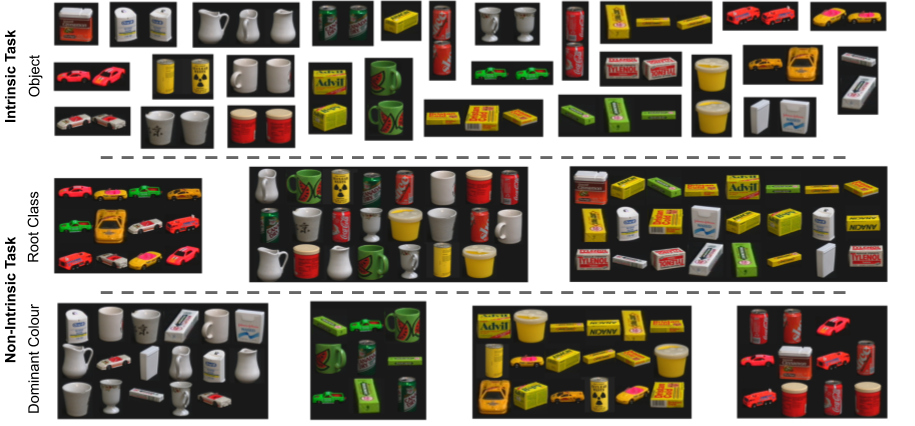
\includegraphics[width=\linewidth]{../files/DMS/images/intrisic_non_intrinsic_white.png}
             \caption{Different clustering tasks using the same data points. The intrinsic task is the most `obvious' division of a dataset this is the task other approaches generally solve. 
             As our method is example-led, it has no bias towards the intrinsic task over other problems.}
    \label{fig__intrisic_non_intrinsic}
\end{figure*}  

\begin{table*}
    \centering     
    \resizebox{\textwidth}{!}{%
\begin{tabular}{ccccccccccccc}	
\hline	
& \multicolumn{3}{c}{\textbf{MNIST}  } & \multicolumn{3}{c}{\textbf{COIL100}  } & \multicolumn{3}{c}{\textbf{YTF} } & \multicolumn{3}{c}{\textbf{RCV1}} \\
\cmidrule(r){2-4} \cmidrule(r){5-7} \cmidrule(r){8-10} \cmidrule(r){11-13}
Algorithms	&	\textbf{ACC}	&	\textbf{NMI}	&	\textbf{AMI}	&	\textbf{ACC}	&	\textbf{NMI}	&	\textbf{AMI}	&	\textbf{ACC}	&	\textbf{NMI}	&	\textbf{AMI}	&	\textbf{ACC}	&	\textbf{NMI}	&	\textbf{AMI}	\\	\hline	
\multicolumn{1}{c}{\textit{Classical} } \\ 
K-means++	&	0.532	&	0.5	&	0.5	&	0.621	&	0.835	&	0.803	&	0.624	&	0.788	&	0.783	&	0.529	&	0.355	&	0.355	\\																					
AC-W	&	0.571	&	0.679	&	0.679	&	0.697	&	0.876	&	0.853	&	0.647	&	0.806	&	0.801	&	0.554	&	0.364	&	0.364	\\																					
DBSCAN	&	0.000	&	0.000	&	0.000	&	0.921	&	0.458	&	0.399	&	0.675	&	0.756	&	0.739	&	0.571	&	0.017	&	0.014	\\																					
SEC	&	0.545	&	0.469	&	0.469	&	0.648	&	0.872	&	0.849	&	0.562	&	0.760	&	0.745	&	0.425	&	0.069	&	0.069	\\																					
LDMGI	&	0.723	&	0.761	&	0.761	&	0.763	&	0.906	&	0.888	&	0.332	&	0.532	&	0.518	&	0.667	&	0.382	&	0.382	\\																
\hline
\multicolumn{1}{c}{\textit{Deep Learning} } \\ 

GDL	&	n/a	&	n/a	&	n/a	&	0.825	&	0.965	&	0.958	&	0.497	&	0.664	&	0.655	&	0.444	&	0.020	&	0.020	\\																					
RCC	&	0.876	&	0.893	&	0.893	&	0.831	&	0.963	&	0.957	&	0.484	&	0.850	&	0.836	&	0.356	&	0.138	&	0.138	\\																					
RCC-DR	&	0.698	&	0.827	&	0.828	&	0.825	&	0.963	&	0.957	&	0.579	&	0.882	&	0.874	&	0.676	&	0.442	&	0.442	\\																					
RCC-DR(SGD)	&	0.696	&	0.827	&	0.827	&	0.855	&	0.967	&	0.961	&	0.473	&	0.845	&	0.830	&	0.354	&	0.106	&	0.106	\\																					


DCN	&	0.560	&	0.570	&	0.570	&	0.600	&	0.830	&	0.810	&	0.620	&	0.810	&	0.790	&	0.730	&	0.470	&	0.470	\\																					
DEC	&	0.867	&	0.853	&	0.840	&	0.815	&	0.645	&	0.611	&	0.643	&	0.811	&	0.807	&	0.683	&	0.504	&	0.500	\\																					
JULE	&	0.800	&	0.900	&	0.900	&	0.911	& 0.983	&	0.979	&	0.342	&	0.587	&	0.574	&	-	&	-	&	-	\\																					
DEPICT	& 0.968	&	0.919	&	0.919	&	0.402	&	0.678	&	0.667	&	0.586	&	0.790	&	0.785	&	-	&	-	&	-	\\																					
DCC	&	0.963	&	0.915	&	0.913	&	0.858	&	0.967	&	0.962	&	0.699	&	0.908	& 0.903	&	0.563	& 0.498 &	0.495	\\																					
\hline	



DMS ($subtract$)
& \textbf{	0.976}	&	\textbf{0.939}	&	\textbf{0.939}	&	\textbf{0.990}	&0.996	&	\textbf{0.994}	& \textbf{0.923}	&\textbf{	0.949}	&	\textbf{0.912}	&	\textbf{0.760}	&	0.587	&	\textbf{0.532}	\\		

DMS ($concat$)
& 0.958		& 0.914		& 0.896		&	\textbf{0.990}	&	\textbf{0.997}	&\textbf{	0.994}	& 0.832		&	0.896	& 0.820		& 0.582	& \textbf{0.603}	&	0.453	\\		


\hline							
\end{tabular}	


}
    \caption{The clustering accuracy of our approach compared against 14 baselines on the intrinsic task of each dataset. Accuracy is measured using the standard accuracy metric (ACC), Normalised Mutual Information (NMI), and Adjusted Mutual Information (AMI).
    Results other than our own are as found in \citet{shah2018deep}.}
\label{table__DMS__results}
\end{table*}

\begin{table*}
\centering
    \resizebox{\textwidth}{!}{%
    
\renewcommand{\arraystretch}{1.2}

 


\begin{tabular}{cccccccccc}
\hline
 & \multicolumn{3}{c}{\textbf{Intrinsic Task} } & \multicolumn{3}{c}{\textbf{Root Class} } & \multicolumn{3}{c}{\textbf{Dominant Colour}}\\
 \cmidrule(r){2-4} \cmidrule(r){5-7} \cmidrule(r){8-10} 
Algorithms & \textbf{ACC} & \textbf{NMI} & \textbf{AMI} & \textbf{ACC} & \textbf{NMI} & \textbf{AMI} & \textbf{ACC} & \textbf{NMI} & \textbf{AMI} \\
\hline
RCC-DR & 0.471 & 0.544 & 0.461 & 0.825 & 0.963 & 0.957 & 0.415 & 0.476 & 0.359 \\
DMS (sub) & \textbf{0.990} & \textbf{0.996} & \textbf{0.994} & \textbf{0.990} & \textbf{0.997} & \textbf{0.996} & \textbf{0.817} & \textbf{0.790} & \textbf{0.751} \\ \hline 
\end{tabular}
    }
    \caption{The ability of our method and other contemporary methods to learn various clustering tasks from the same COIL100 features. 
    All tasks use the same features,
    but the clustering focuses on a different aspect of the semantic information.}
\label{table__DMS__redefined_task}
\end{table*}


    
\subsection{Ablation} 
\label{sec__DMS__ablation} 

In this section, we evaluate components of our training approach and network architecture. We vary the number of mean shift iterations used during training, the number of layers used in the kernel, and the robustness of subtraction and concatenation-based kernels to limited training data.

\subsubsection{Training Iterations}

The optimal performance of DMS is when 4 iterations are used during the training of our kernel; the comparison to other numbers of iterations are shown in \Cref{table__DMS__ablation_training_iteration}.
We hypothesise that when a small number of iterations are used, the network does not have sufficient flexibility to learn the nuance of the given task. 
Conversely, with a large number of iterations, the network is not incentivised to effectively define the clusters as it has many opportunities to improve its prediction. 
We found that the number of iterations required for convergence at inference time increased proportionally with both the number of training iterations and the complexity of the dataset. 
This verifies the idea that a single pass through the kernel is less able to distinguish inliers from outliers given more training iterations.
Given four training iterations, the time taken to converge at inference time varied between one and five iterations depending on the complexity of the dataset.


\subsubsection{Kernel Depth} 

Here, we evaluate the effect of varying the number of fully connected layers used in the differentiable kernel.
All networks are trained for the same number of epochs.
We use a sufficient number of epochs to ensure the training of all networks had converged. 
As shown in \Cref{table__DMS__ablation_fully_connected}, increasing the depth of the kernel improves the performance of the method.
After three layers, the performance improvements are negligible while training time and likelihood of overfitting increase. For this reason, we use three fully connected layers for all other tests.

\subsubsection{Concatenation and Subtraction Kernels}\label{sec__DMS__ablation_sub_cat_kernels}

Here, we test two differentiable kernels, the subtraction-based kernel,
which takes the difference of the data point and sample mean, $(\mathbf{x} - \bar{\boldsymbol{\mu}}_i)$, and an alternative concatenation-based kernel, which takes a concatenation of the data point and sample mean, $concat(\mathbf{x}, \bar{\boldsymbol{\mu}}_i)$.
The concatenation kernel requires the addition of an extra fully-connected layer compared to the subtraction-based kernel. We use the same architecture as the original differential kernel after this. 

While we hypothesised the use of a concatenation and a fully-connected layer would be more effective than the simpler subtraction as a greater amount of information could be used, this turned out to not be the case. As shown in \Cref{table__DMS__results}, the results of both kernels were comparable on datasets where it was likely all clusters would be represented. However, the results varied significantly when this was not the case. It should be noted that the concatenation and the additional first layer could simply learn the subtraction function. 


    \begin{table}
        \centering         


\begin{tabular}{cccc}
\hline
Layers  & ACC & NMI & AMI \\
\hline
2 & 0.818 & 0.920 & 0.847 \\
4 & \textbf{0.923} & \textbf{0.949} & \textbf{0.912} \\
6 & 0.890 & 0.915 & 0.883 \\
8 & 0.780 & 0.837 & 0.813 \\
\hline
\end{tabular}










        \caption{The performance of our differentiable kernel with varied training iterations on the YTF dataset.}
    \label{table__DMS__ablation_training_iteration}
    \end{table}
    
    \begin{table}
        \centering        
        
\begin{tabular}{cccc}
\hline
Layers  & ACC & NMI & AMI \\
\hline
1 & 0.069 & 0.000 & 0.000\\
2 & 0.920 & 0.934 & 0.895 \\
3 & \textbf{0.923} & 0.939 & \textbf{0.912}\\
4 & 0.905 & \textbf{0.942} & 0.898\\
\hline
\end{tabular}
        \caption{The performance of our differentiable kernel with a varied number of fully connected layers on the YTF dataset.}
    \label{table__DMS__ablation_fully_connected}
    \end{table}
    

As it is clear that the concatenation-based kernel performs worse than the subtraction-based kernel on more sparse datasets, we further test their performance when less side-information is available. 
Here, unlike our other experiments where the points with side-information are randomly selected, we explicitly limit the number of classes and points per class with side-information.
The results of this experiment appear in \Cref{fig__DMS__class_and_points}. 

The performance of both kernels degrades similarly when fewer data points per class are seen during training. There is little effect on the performance unless the number of data points is significantly restricted. 
However, while the concatenation-based kernel performs better in cases where all of the ground-truth classes are present in the training data, its performance is significantly reduced when this is not the case.


\begin{figure}
 \centering
            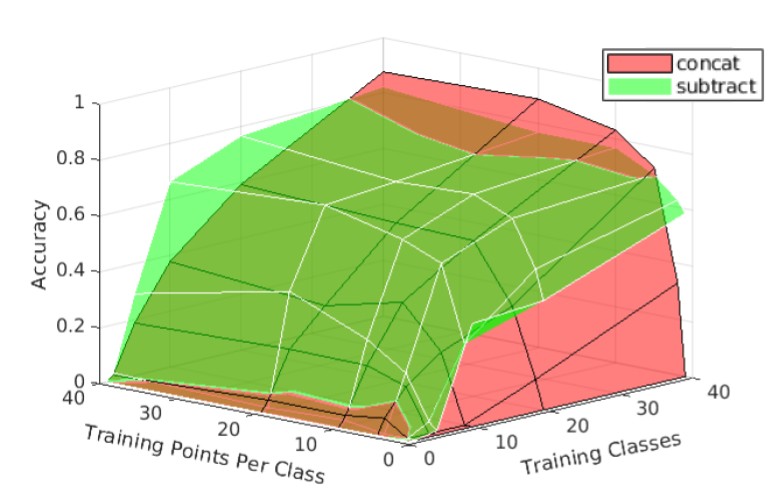
\includegraphics[width=0.5\linewidth]{../files/DMS/images/clpgraph.png}
            \caption{The effect of varying the distribution of training data on the performance of our subtraction and convolution-based kernels.
             For this test, we explicitly limit the number of classes and the maximum number of points per class with side-information during training.
             This shows the method's ability to discover novel classes as there is very little decrease in performance of the subtraction-based method when half of the classes are absent during training.}
    \label{fig__DMS__class_and_points}
 \end{figure} 
 
The subtraction-based kernel, on the other hand, has little degradation in performance when decreasing the classes present during training, which demonstrates that it is better able to generalise to unseen data.
We believe this is because the subtraction-based kernel, unlike the concatenation kernel, is only presented with the relative position of points to the current sample mean estimate. 
During training, the subtraction-based kernel is unable to use the global position of the training clusters as a crutch and must learn to find a better description of similarity.  
This experiment clearly shows the method's ability to correctly identify and cluster novel classes, as both kernels maintain high accuracy when $\sim 75\%$ of the classes are not present during training.


\section{Conclusion}\label{DMS__sec__conclusion}
In this chapter, we present a novel approach to clustering which learns to cluster points directly from side-information in the form of pairwise similarity. 
Unlike previous work, this approach does not require any other knowledge of the dataset as a whole; it does not require knowledge of the number of clusters, their centres, or any kind of distance metric as a prior.
We demonstrate this approach using DMS, a differential, iterative clustering method inspired by the mean shift algorithm. 

DMS learns the requirements of a task and uses this to outperform state-of-the-art deep-learning-based clustering approaches on both intrinsic and non-intrinsic tasks without the need to specify any task or dataset-specific hyper-parameters.
This flexibility, along with DMS's performance in high-dimensional feature spaces and its lightweight nature, enables it to be seamlessly incorporated into other deep learning applications for end-to-end training or as a head on top of an already trained backbone.

It should be noted that the work presented in this chapter was completed soon after the introduction of the attention mechanism and before the introduction of the vision transformer.
While using attention mechanisms for clustering is difficult due to their $\mathcal{O}(n)$ complexity, we believe that utilising an attention mechanism in the kernel on a subset of inlier points to further refine inlier predictions would likely improve our method's accuracy.

While the identification of similarity that DMS provides is crucial for counting, it is limited to counting separately provided instances.
Most of the current computer vision literature defines counting as the identification \textit{and} enumeration of similar instances within an image rather than the enumeration of already separated instances in distinct images.
In order to use DMS in these settings, an additional detection or segmentation stage would be required.
Instead of implementing a two-stage detect-then-count framework, we go on to focus on addressing both stages simultaneously to develop a single-stage exemplar free class-agnostic counter.









\end{document}